\chapter{Results}
\label{ch:results}

This chapter reports what the analyses found. Interpretation is held back for Chapter~\ref{ch:discussion}; here the tables and figures carry the numbers and the prose says what each shows. Every value is a macro generated from the result files, every rate is read against its random-pairing null (\nullShuffles{} re-pairings, seed \nullSeed), and every interval is a clustered bootstrap over prompt groups (\DiffDraws{} draws).

\section{Overall agreement}
\label{sec:results-overall}

Table~\ref{tab:headline} gives the four measures on the \nEmotional{} prompts the text reader labels emotional, and Figure~\ref{fig:zgroup} shows the same cells as distances from their nulls. Every measure sits well above chance. Valence-sign agreement is \FullEmoSignObs{} against a null of \FullEmoSignNull{} ($z$ = \FullEmoSignZ{}, 95\% CI \FullEmoSignCi{}); the denominator is \FullEmoNSign{} rather than \FullEmoN{}, because prompts whose top family is surprise have no valence sign. Family agreement is \FullEmoFamObs{} against \FullEmoFamNull{} ($z$ = \FullEmoFamZ{}, CI \FullEmoFamCi{}), top-3 overlap \FullEmoOvlpObs{} against \FullEmoOvlpNull{} ($z$ = \FullEmoOvlpZ{}), and valence--arousal similarity \FullEmoVaObs{} against \FullEmoVaNull{} ($z$ = \FullEmoVaZ{}). The loosest measure has the largest $z$ and the smallest gap in percentage points, which is the floor of Equation~\ref{eq:va} at work: its null is high and tight, so a modest excess over it is many standard deviations.

% GENERATED by emoviz/export_tex.py — do not edit
\begin{table}[htbp]
\centering
\small
\caption{Agreement between the prompt reader and the image reader on the 1,012 analysed records, by prompt group and image class, against the random-pairing null (300 re-pairings, seed 7). CI: clustered bootstrap over prompt groups (10,000 draws). n/a: degenerate null (every prompt in the subset shares one label, so permutation cannot change the score).}
\label{tab:headline}
\begin{tabular}{lrrrl}
\toprule
Subset / measure & Observed & Null & $z$ & 95\% CI \\
\midrule
\textbf{Emotional prompts} ($n$=607; sign $n$=530) &  &  &  &  \\
Valence--arousal similarity & 83.8\% & 77.3\% & +12.2 & [82.0, 85.5] \\
Valence-sign agreement & 64.0\% & 45.6\% & +11.1 & [58.6, 68.8] \\
Family agreement & 53.0\% & 38.8\% & +10.3 & [47.3, 58.7] \\
Top-3 soft overlap & 50.6\% & 39.4\% & +11.6 & [46.5, 54.7] \\
\midrule
\textbf{\quad face-classified} ($n$=402; sign $n$=360) &  &  &  &  \\
Valence--arousal similarity & 84.2\% & 76.4\% & +11.2 & [82.3, 86.1] \\
Valence-sign agreement & 73.9\% & 53.5\% & +10.4 & [68.3, 79.2] \\
Family agreement & 61.9\% & 45.8\% & +10.3 & [55.8, 68.0] \\
Top-3 soft overlap & 53.4\% & 40.4\% & +11.6 & [49.2, 57.7] \\
\midrule
\textbf{\quad scene-classified} ($n$=205; sign $n$=170) &  &  &  &  \\
Valence--arousal similarity & 82.9\% & 79.1\% & +6.0 & [80.4, 85.2] \\
Valence-sign agreement & 42.9\% & 29.6\% & +5.8 & [33.1, 51.1] \\
Family agreement & 35.6\% & 26.2\% & +4.4 & [26.4, 44.1] \\
Top-3 soft overlap & 44.9\% & 38.1\% & +4.9 & [38.7, 51.0] \\
\midrule
\textbf{Neutral-labelled prompts} ($n$=405; sign $n$=0) &  &  &  &  \\
Valence--arousal similarity & 76.6\% & 76.6\% & +0.3 & [75.6, 77.6] \\
Valence-sign agreement & 0.0\% & 0.0\% & n/a & degenerate \\
Family agreement & 28.6\% & 28.6\% & n/a & degenerate \\
Top-3 soft overlap & 31.6\% & 31.6\% & +0.0 & -- \\
\bottomrule
\end{tabular}
\end{table}


\begin{figure}[htbp]
\centering
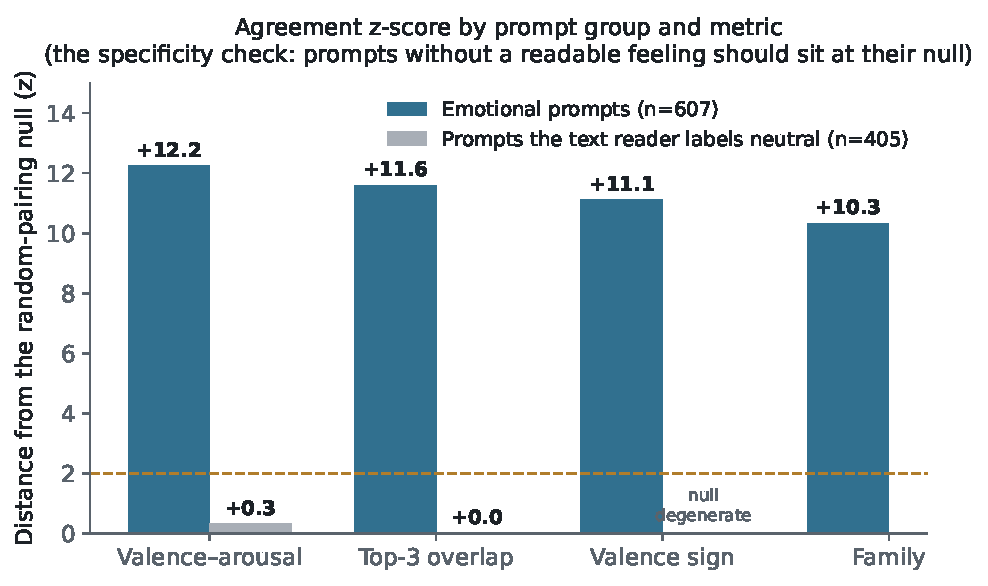
\includegraphics[width=0.9\textwidth]{fig3_z_by_prompt_group}
\caption{Distance from the random-pairing null ($z$) by prompt group and measure. For the neutral-labelled prompts the sign and family nulls are degenerate and no $z$ is shown.}
\label{fig:zgroup}
\end{figure}

\section{Face-classified versus scene-classified drawings}
\label{sec:results-face-scene}

Figure~\ref{fig:facescene} and Table~\ref{tab:difference} split the emotional prompts by the describer's image class. On the \FullFaceN{} face-classified records valence-sign agreement is \FullFaceSignObs{} against a null of \FullFaceSignNull{} ($z$ = \FullFaceSignZ{}, CI \FullFaceSignCi{}) and family agreement \FullFaceFamObs{} against \FullFaceFamNull{} ($z$ = \FullFaceFamZ{}). On the \FullSceneN{} scene-classified records the same measures are \FullSceneSignObs{} against \FullSceneSignNull{} ($z$ = \FullSceneSignZ{}, CI \FullSceneSignCi{}) and \FullSceneFamObs{} against \FullSceneFamNull{} ($z$ = \FullSceneFamZ{}). Both classes clear their nulls in this table; Section~\ref{sec:results-ablation} returns to the scene row.

The two nulls differ, so the contrast is stated as a difference rather than a ratio. Face minus scene is \DiffSignPp{} on valence-sign agreement (CI \DiffSignCi{}) and \DiffFamPp{} on family agreement (CI \DiffFamCi{}), with the clustered permutation test giving $p$ = \DiffSignP{} on both. Valence--arousal similarity does not separate the classes (\FullFaceVaObs{} against \FullSceneVaObs{}); the difference lives in the categorical rungs.

\begin{figure}[htbp]
\centering
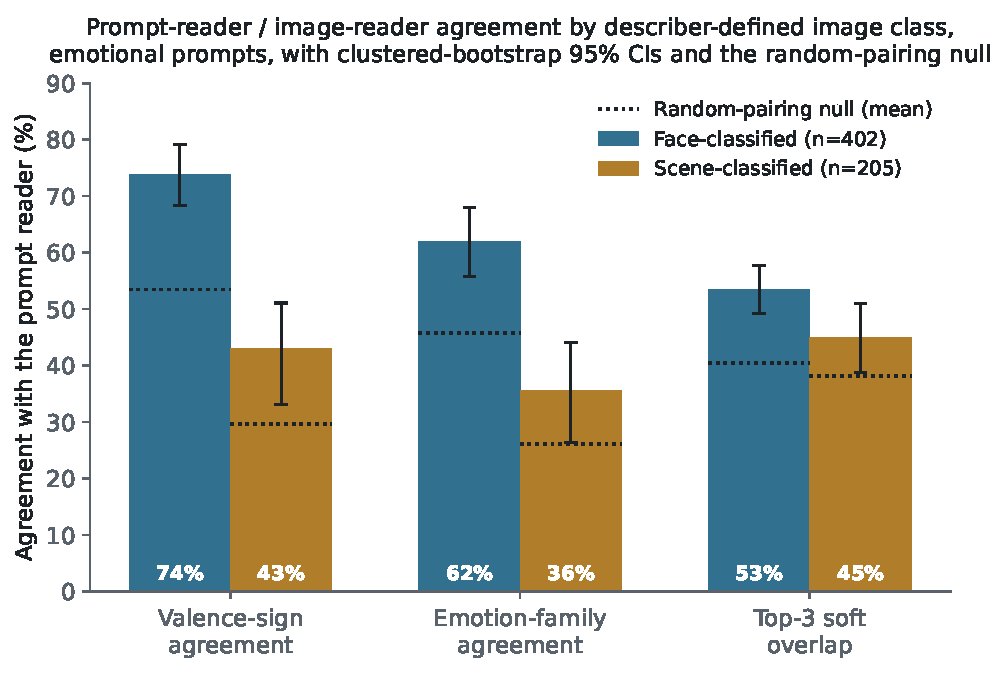
\includegraphics[width=\textwidth]{fig1_face_vs_scene}
\caption{Agreement between the prompt reader and the image reader on the emotional prompts, by describer-defined image class, with clustered-bootstrap 95\% CIs (error bars) and each cell's random-pairing null (dotted).}
\label{fig:facescene}
\end{figure}

% GENERATED by emoviz/export_tex.py — do not edit
\begin{table}[htbp]
\centering
\footnotesize
\caption{Face-classified versus scene-classified drawings on the emotional prompts: agreement with 95\% clustered-bootstrap CIs, the difference with its CI, and the clustered permutation p (10,000 draws; significance.py).}
\label{tab:difference}
\begin{tabular}{lllll}
\toprule
Measure & Face ($n$=402) & Scene ($n$=205) & Difference (pp) & Perm.\ $p$ \\
\midrule
Valence-sign agreement & 73.9\% [68.3, 79.2] & 42.9\% [33.1, 51.1] & +30.9~pp [+22.6, +40.6] & 0.0001 \\
Family agreement & 61.9\% [55.8, 68.0] & 35.6\% [26.4, 44.1] & +26.3~pp [+18.4, +35.3] & 0.0001 \\
\bottomrule
\end{tabular}
\end{table}


\section{Robustness to repeated prompts and multiple comparisons}
\label{sec:results-robustness}

Table~\ref{tab:distinct} recomputes the main table on the first occurrence of each prompt, \nDistinct{} records of which \nDistinctEmo{} are emotional. The overall and face results hold: on the \DistFaceN{} distinct face-classified records valence-sign agreement is \DistFaceSignObs{} ($z$ = \DistFaceSignZ{}) and family agreement \DistFaceFamObs{} ($z$ = \DistFaceFamZ{}). The scene result weakens substantially: valence-sign agreement falls to \DistSceneSignObs{} ($z$ = \DistSceneSignZ{}) and family agreement to \DistSceneFamObs{} ($z$ = \DistSceneFamZ{}) on \DistSceneN{} records.

Table~\ref{tab:holm} applies the Holm--Bonferroni procedure to the \HolmM{} non-degenerate $z$-scores the analysis prints. \HolmSurvive{} survive at family-wise 0.05 and \HolmFail{} do not. Every full-sample cell on the emotional, face and scene subsets survives, as does every distinct-prompt cell on the emotional and face subsets. The cells that fail are the ones expected to sit at chance (the neutral-labelled control on both blocks), the single-valence subsets' valence--arousal and overlap cells, and the distinct-prompt scene family cell ($z$ = \DistSceneFamZ{}), which should be read as suggestive rather than established.

% GENERATED by emoviz/export_tex.py — do not edit
\begin{table}[htbp]
\centering
\small
\caption{The same analysis on the 763 distinct prompts only (first occurrence of each prompt text kept), a check against pseudo-replication from the 249 repeated prompts.}
\label{tab:distinct}
\begin{tabular}{lrrrl}
\toprule
Subset / measure & Observed & Null & $z$ & 95\% CI \\
\midrule
\textbf{Emotional prompts} ($n$=452; sign $n$=394) &  &  &  &  \\
Valence--arousal similarity & 83.0\% & 76.5\% & +10.6 & [81.5, 84.4] \\
Valence-sign agreement & 62.2\% & 44.4\% & +9.9 & [57.2, 67.0] \\
Family agreement & 51.3\% & 37.2\% & +9.3 & [46.7, 56.0] \\
Top-3 soft overlap & 48.9\% & 37.7\% & +10.8 & [45.9, 51.9] \\
\midrule
\textbf{\quad face-classified} ($n$=319; sign $n$=284) &  &  &  &  \\
Valence--arousal similarity & 83.5\% & 75.5\% & +9.7 & [81.7, 85.2] \\
Valence-sign agreement & 71.8\% & 51.0\% & +8.4 & [66.4, 77.0] \\
Family agreement & 59.9\% & 43.0\% & +8.1 & [54.2, 65.2] \\
Top-3 soft overlap & 51.8\% & 38.4\% & +9.7 & [48.1, 55.4] \\
\midrule
\textbf{\quad scene-classified} ($n$=133; sign $n$=110) &  &  &  &  \\
Valence--arousal similarity & 81.8\% & 78.9\% & +3.6 & [79.5, 83.8] \\
Valence-sign agreement & 37.3\% & 27.1\% & +3.5 & [28.1, 46.2] \\
Family agreement & 30.8\% & 24.1\% & +2.6 & [23.3, 38.4] \\
Top-3 soft overlap & 41.7\% & 36.7\% & +3.1 & [36.9, 46.5] \\
\midrule
\textbf{Neutral-labelled prompts} ($n$=311; sign $n$=0) &  &  &  &  \\
Valence--arousal similarity & 76.6\% & 76.4\% & +1.1 & -- \\
Valence-sign agreement & 0.0\% & 0.0\% & n/a & degenerate \\
Family agreement & 27.7\% & 27.7\% & n/a & degenerate \\
Top-3 soft overlap & 31.4\% & 31.1\% & +0.8 & -- \\
\bottomrule
\end{tabular}
\end{table}

% GENERATED by emoviz/export_tex.py — do not edit
\begin{table}[htbp]
\centering
\footnotesize
\caption{Multiple-comparison control over the 36 non-degenerate $z$-scores the analysis prints (12 degenerate ones excluded). Two-sided $p$ by the normal approximation; Holm--Bonferroni at family-wise 0.05: 26 survive, 10 do not.}
\label{tab:holm}
\begin{tabular}{lp{0.78\textwidth}}
\toprule
Outcome & Tests \\
\midrule
Do not survive & DISTINCT negative prompts overlap z+2.7; DISTINCT scene images family z+2.6; FULL positive prompts overlap z+2.3; FULL negative prompts va z+2.1; DISTINCT positive prompts overlap z+1.9; DISTINCT negative prompts va z+1.6; DISTINCT non-emotional va z+1.1; DISTINCT non-emotional overlap z+0.8; FULL non-emotional va z+0.3; FULL non-emotional overlap z+0.0 \\
Survive & the remaining 26, including every headline (emotional, face and scene on all four measures; distinct-prompt emotional and face) \\
\bottomrule
\end{tabular}
\end{table}


\section{Specificity check: prompts the text reader labels neutral}
\label{sec:results-control}

On the \CtrlN{} prompts the text reader labels neutral, only the valence--arousal measure has a live null. It sits on it: \CtrlVaObs{} observed against \CtrlVaNull{} expected ($z$ = \CtrlVaZ{} at record level, \CtrlVaZClustered{} against a null clustered on prompt groups). Family agreement equals its null exactly (\CtrlFamObs{}) because every prompt in the subset shares the neutral label, so permutation cannot move it; the same holds for valence sign, whose numerator and denominator are both zero here.

The control audit (Table~\ref{tab:control}) qualifies the set. \CtrlFlagged{} of the \CtrlN{} prompts (\CtrlFlaggedPct{}) contain a plain English affect word from a fixed \CtrlLexicon{}-word lexicon, most often \CtrlTopWords{}; \CtrlNameOnly{} consist of a redacted name alone. On the cleaned control of \CtrlCleanN{} records the result is unchanged: \CtrlCleanVaObs{} against \CtrlCleanVaNull{} ($z$ = \CtrlCleanVaZ{}). The null's spread on this subset is very small (\CtrlVaSd{}) because the prompt-side points barely vary, so observed and expected values are expected to coincide here; the check is passed, and it is a weak one.

% GENERATED by emoviz/export_tex.py — do not edit
\begin{table}[htbp]
\centering
\small
\caption{The specificity check on the prompts the text reader labels neutral. Only valence--arousal similarity is informative there (sign and family are degenerate: every prompt shares the neutral label). Cleaned control = minus the 2 records reduced to `[name]' and the 68 containing one of 66 plain affect words.}
\label{tab:control}
\begin{tabular}{lrrrrr}
\toprule
Control set & $n$ & VA observed & VA null & $z$ (record null) & $z$ (clustered null) \\
\midrule
All neutral-labelled prompts & 405 & 76.6\% & 76.5\% & +0.5 & -0.1 \\
Cleaned control & 335 & 76.6\% & 76.6\% & +0.0 & -0.6 \\
\bottomrule
\end{tabular}
\end{table}


\section{Two image readers, like for like}
\label{sec:results-method}

Figure~\ref{fig:method} and Table~\ref{tab:method} score two image readers against the same prompt reader on the same \McN{} emotional records with the same measures and the same random re-pairings. Describe-then-extract agrees with the prompt reader on \McDeFam{} of families against \McClipFam{} for direct CLIP, a difference of \McDiffFamPp{} (CI \McDiffFamCi{}); the cluster sign-flip test gives $p$ \McClusterFamP{}, and the unclustered exact McNemar test, which treats records as independent and is optimistic, gives $p$ = \McMcNemarFamP{}. On valence sign the figures are \McDeSign{} against \McClipSign{} (\McDiffSignPp{}, CI \McDiffSignCi{}); on overlap \McDeOvlp{} against \McClipOvlp{}; on valence--arousal similarity \McDeVa{} against \McClipVa{}. Of the \McN{} records, \McFamB{} are ones only describe-then-extract agrees on and \McFamC{} ones only direct CLIP agrees on; \McFamBoth{} are agreed by both and \McFamNeither{} by neither.

Two details in the table need saying. Direct CLIP's family $z$ (\McClipFamZ{}) is higher than describe-then-extract's (\McDeFamZ{}) although its rate is far lower, because its null is lower and tighter: it reads \McClipNeutral{} of the \McN{} images as neutral, so it rarely agrees by chance either. The $z$ measures distance from chance, not level of agreement, and the paired tests on the rates are the comparison. And the two image readers agree with each other on only \McReaderAgree{} of top-1 families. Table~\ref{tab:methodvone} reproduces the comparison from the first build (\McVOneN{} records, an entailment reader on the prompt side, a different overlap formula), kept as a record; it is not comparable with the main analysis and its figures are not quoted.

\begin{figure}[htbp]
\centering
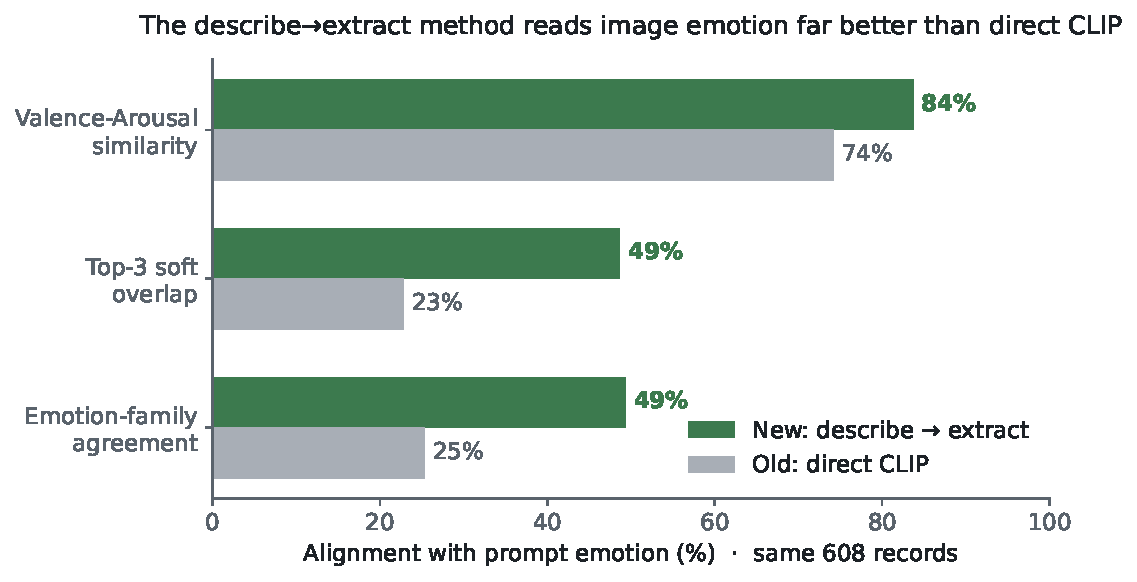
\includegraphics[width=\textwidth]{fig2_method_comparison}
\caption{Two image readers scored against the same prompt reader on the same \McN{} emotional records, each against its own random-pairing null (dotted).}
\label{fig:method}
\end{figure}

% GENERATED by emoviz/export_tex.py — do not edit
\begin{table}[htbp]
\centering
\scriptsize
\caption{Two image readers scored like for like against the same prompt reader (GoEmotions) on the same 607 emotional records with the same measures and the same 300 re-pairings. $b$ = records only describe-then-extract agrees on; $c$ = records only direct CLIP agrees on. The exact McNemar $p$ treats records as independent and is optimistic ($3.4\times10^{-35}$ for family); the cluster sign-flip randomisation (20,000 draws) respects prompt groups.}
\label{tab:method}
\begin{tabular}{lrrrrrr}
\toprule
Measure & Describe→extract & null & $z$ & Direct CLIP & null & $z$ \\
\midrule
Valence--arousal similarity & 83.8\% & 77.3\% & +12.2 & 73.3\% & 70.1\% & +10.2 \\
Valence-sign agreement & 64.0\% & 45.6\% & +11.1 & 31.1\% & 18.6\% & +9.9 \\
Family agreement & 53.0\% & 38.8\% & +10.3 & 22.4\% & 12.2\% & +11.1 \\
Top-3 soft overlap & 50.6\% & 39.4\% & +11.6 & 26.4\% & 20.2\% & +11.2 \\
\midrule
Paired family test & $b$=218, $c$=32 &  &  & diff +30.6~pp & CI [+25.5, +35.6] & cluster $p<0.001$ \\
Paired valence-sign test & $b$=204, $c$=30 &  &  & diff +32.8~pp & CI [+27.4, +38.2] & cluster $p<0.001$ \\
\bottomrule
\end{tabular}
\end{table}

% GENERATED by emoviz/export_tex.py — do not edit
\begin{table}[htbp]
\centering
\small
\caption{The earlier (v1) comparison as published in the build log: prompt side read by BART-MNLI, the 608 records of the v1 lexicon rule, and a different overlap formula. Kept as a record; not comparable with Table~\ref{tab:headline}.}
\label{tab:methodvone}
\begin{tabular}{lrr}
\toprule
Measure & Describe→extract & Direct CLIP \\
\midrule
Family agreement & 49.3\% & 25.3\% \\
Top-3 soft overlap & 48.6\% & 22.8\% \\
Valence--arousal similarity & 83.7\% & 74.2\% \\
\bottomrule
\end{tabular}
\end{table}


\section{Consistency across repeated prompts}
\label{sec:results-consistency}

\nGroups{} prompts were drawn two or more times, covering \nGroupRecords{} records; \nPairGroups{} of the groups are pairs. Figure~\ref{fig:consistency} and Table~\ref{tab:consistency} give the within-group agreement of the image reader. The mean share of drawings in a group that receive the group's modal family is \ConsFam{} (CI over groups \ConsFamCi{}) against a permutation null of \ConsFamNull{} (sd \ConsFamNullSd{}), $z$ = \ConsFamZ{}, permutation $p$ = \ConsFamP{}. The same valence sign is returned for \ConsVal{} of drawings within a group against \ConsValNull{} ($z$ = \ConsValZ{}). \ConsFull{} of the \nGroups{} groups (\ConsFullPct{}) are fully consistent, every drawing receiving one family, against \ConsFullNull{} expected ($z$ = \ConsFullZ{}). The largest group, the word ``happy'' drawn \ConsHappyN{} times, was read as joy \ConsHappyJoy{} times, neutral \ConsHappyNeutral{} times and surprise \ConsHappySurprise{} once.

\begin{figure}[htbp]
\centering
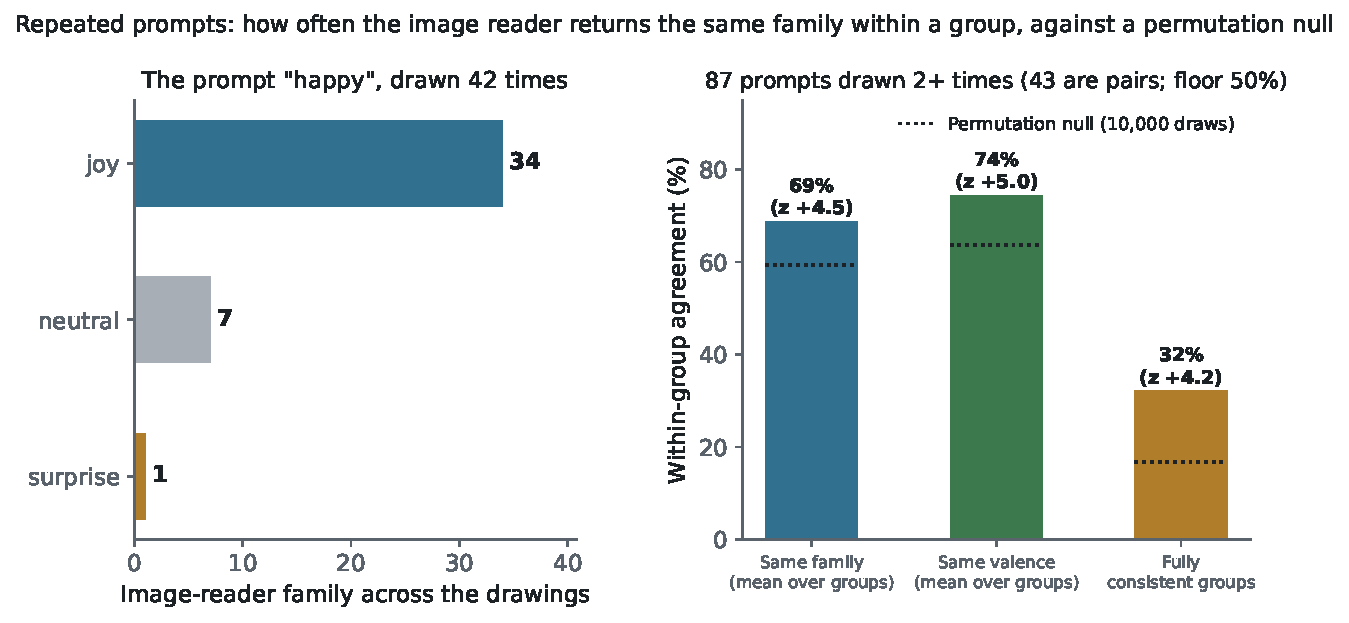
\includegraphics[width=\textwidth]{fig4_consistency}
\caption{Repeated prompts: the image reader's top-1 family across the \ConsHappyN{} drawings of ``happy'' (left), and within-group agreement over all \nGroups{} repeated prompts against the permutation null (right).}
\label{fig:consistency}
\end{figure}

% GENERATED by emoviz/export_tex.py — do not edit
\begin{table}[htbp]
\centering
\small
\caption{Within-group agreement of the image reader across the 87 prompts drawn two or more times (336 records; 43 groups are pairs, whose modal agreement cannot fall below 50\%), against a permutation null that shuffles the image readings over all 1,012 analysed records and re-cuts them into the same groups (10,000 draws, seed 7).}
\label{tab:consistency}
\begin{tabular}{lrrrr}
\toprule
Quantity & Observed & Null mean (sd) & $z$ & $p$ \\
\midrule
Same family, mean over groups & 68.8\% & 59.4\% (2.1\%) & +4.5 & $1.0\times10^{-4}$ \\
Same valence, mean over groups & 74.5\% & 63.7\% (2.1\%) & +5.0 & $1.0\times10^{-4}$ \\
Fully consistent groups (of 87) & 28 & 14.5 (3.2) & +4.2 & $2.0\times10^{-4}$ \\
\bottomrule
\end{tabular}
\end{table}


\section{Per-family agreement}
\label{sec:results-families}

Figure~\ref{fig:confusion} and Table~\ref{tab:confusion} cross the prompt reader's family with the image reader's on the \nEmotional{} emotional records; Table~\ref{tab:families} gives the marginals over all \nAnalysed{} analysed records. The prompt side is dominated by joy (\RecJoyN{} of the emotional prompts), with sadness (\RecSadnessN{}) and surprise (\RecSurpriseN{}) next and fear (\RecFearN{}), anger (\RecAngerN{}) and disgust (\RecDisgustN{}) rare. Recall by prompt family, meaning the share of prompts in a family whose drawing the image reader placed in the same family, is \RecJoy{} for joy (CI \RecJoyCi{}), \RecSadness{} for sadness (CI \RecSadnessCi{}), \RecAnger{} for anger on \RecAngerN{} prompts, \RecSurprise{} for surprise (CI \RecSurpriseCi{}), and \RecFear{} for fear on \RecFearN{} prompts. Across all \nAnalysed{} records the image reader never returns disgust and returns fear \famImageFear{} times.

Cohen's kappa for family agreement (Table~\ref{tab:kappa}) is \KappaEmo{} on the emotional prompts (CI \KappaEmoCi{}), \KappaFace{} on the face-classified records and \KappaScene{} on the scene-classified: \KappaEmoBand{}, \KappaFaceBand{} and \KappaSceneBand{} on the Landis--Koch scale. In practice the seven-family ladder is a three-family one, joy, sadness and neutral, with anger a distant fourth; the remaining families are too rare on the prompt side, or never produced on the image side, to support any claim.

\begin{figure}[htbp]
\centering
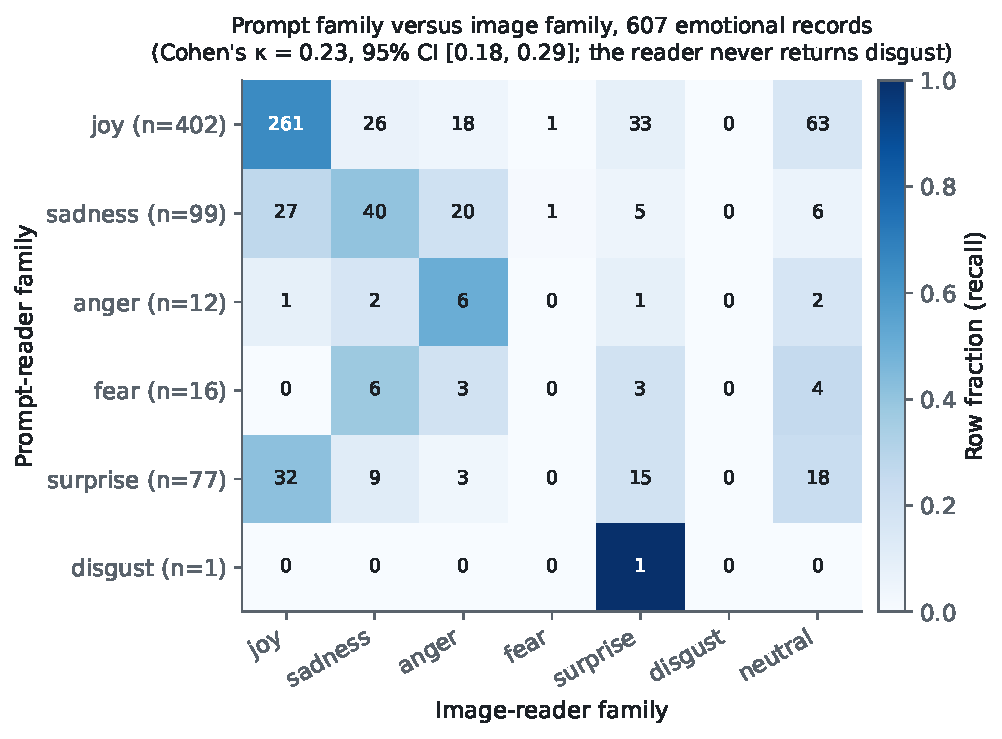
\includegraphics[width=0.85\textwidth]{fig6_confusion}
\caption{Prompt-reader family (rows) against image-reader family (columns) on the \nEmotional{} emotional records; cell = count, shading = row fraction.}
\label{fig:confusion}
\end{figure}

% GENERATED by emoviz/export_tex.py — do not edit
\begin{table}[htbp]
\centering
\scriptsize
\caption{Prompt-reader family (rows) against image-reader family (columns) on the 607 emotional records. Recall = row diagonal share, with a clustered-bootstrap 95\% CI. Cohen's $\kappa$ = 0.23 [0.18, 0.29]. The image reader never returns disgust and returns fear 4 times in 1,012 records.}
\label{tab:confusion}
\begin{tabular}{lrrrrrrrrl}
\toprule
Prompt \textbackslash{} image & joy & sadness & anger & fear & surprise & disgust & neutral & $n$ & Recall [CI] \\
\midrule
joy & 261 & 26 & 18 & 1 & 33 & 0 & 63 & 402 & 64.9\% [59, 70] \\
sadness & 27 & 40 & 20 & 1 & 5 & 0 & 6 & 99 & 40.4\% [31, 51] \\
anger & 1 & 2 & 6 & 0 & 1 & 0 & 2 & 12 & 50.0\% [22, 78] \\
fear & 0 & 6 & 3 & 0 & 3 & 0 & 4 & 16 & 0.0\% [0, 0] \\
surprise & 32 & 9 & 3 & 0 & 15 & 0 & 18 & 77 & 19.5\% [11, 28] \\
disgust & 0 & 0 & 0 & 0 & 1 & 0 & 0 & 1 & 0.0\% [0, 0] \\
\midrule
\textit{image total} & 321 & 83 & 50 & 2 & 58 & 0 & 93 & 607 &  \\
\bottomrule
\end{tabular}
\end{table}

% GENERATED by emoviz/export_tex.py — do not edit
\begin{table}[htbp]
\centering
\small
\caption{Cohen's $\kappa$ for family agreement (7 families), with clustered-bootstrap 95\% CIs and the Landis \& Koch (1977) band. The neutral-labelled subset is degenerate ($\kappa$ = 0 by construction) and is omitted.}
\label{tab:kappa}
\begin{tabular}{lrrll}
\toprule
Subset & $n$ & $\kappa$ & 95\% CI & Band \\
\midrule
emotional & 607 & 0.23 & [0.18, 0.29] & fair \\
face & 402 & 0.30 & [0.23, 0.37] & fair \\
scene & 205 & 0.13 & [0.06, 0.19] & slight \\
all analysed & 1012 & 0.21 & [0.16, 0.25] & fair \\
distinct emotional & 452 & 0.23 & [0.17, 0.29] & fair \\
distinct face & 319 & 0.29 & [0.21, 0.37] & fair \\
distinct scene & 133 & 0.09 & [0.01, 0.17] & slight \\
\bottomrule
\end{tabular}
\end{table}

% GENERATED by emoviz/export_tex.py — do not edit
\begin{table}[htbp]
\centering
\small
\caption{Top-1 family marginals of the two readers over all 1,012 analysed records.}
\label{tab:families}
\begin{tabular}{lrr}
\toprule
Family & Prompt reader & Image reader \\
\midrule
joy & 402 & 461 \\
sadness & 99 & 141 \\
anger & 12 & 89 \\
fear & 16 & 4 \\
surprise & 77 & 108 \\
disgust & 1 & 0 \\
neutral & 405 & 209 \\
\bottomrule
\end{tabular}
\end{table}


\section{The describer}
\label{sec:results-describer}

Table~\ref{tab:describer} crosses the describer's people count with the presence of an expression word over all \nAnalysed{} records. The describer answers the expression question for every drawing. It returns an expression word for \DescNoPeopleExpr{} of the records in which it simultaneously reports that no people are present. Of the \DescSceneN{} scene-classified records, \DescScenePeopleZero{} report no people; \DescScenePeopleZeroExpr{} of those still carry an expression word, and \DescSceneSmile{} answer ``smile'', ``smiling'' or ``happy'' (\DescSceneSmilePct{} of the no-people records). The smile rate depends on the denominator and is given with both: \DescSmileFace{} of the \nFaceAll{} face-classified records and \DescSmileAll{} of all \nAnalysed{} analysed records.

The copy rate measures how much the extraction stage adds to the describer's own word. Where the expression answer names an emotion outright (\DescBareStrictN{} records, \DescBareStrictPct{} of the corpus), the image reader's top-1 family equals the family that word implies \DescCopyStrict{} of the time. On the broad definition, which admits facial actions such as ``smile'' and ``crying'', the copy rate is \DescCopyBroad{}: \DescCopyBroadPeople{} where a person is reported and \DescCopyBroadPeopleZero{} where none is, the ``0 people'' token pulling the reading towards neutral.

% GENERATED by emoviz/export_tex.py — do not edit
\begin{table}[htbp]
\centering
\small
\caption{The describer's answers on all 1,012 analysed records: people count crossed with whether the facial-expression answer contains an expression word. The face rule is the top-left cell. Of the 421 scene-classified records, 414 report no people and 406 of those still contain an expression word (332 answer smile, smiling or happy).}
\label{tab:describer}
\begin{tabular}{lrr}
\toprule
 & Expression word present & Expression word absent \\
\midrule
People $\geq 1$ & 591 & 7 \\
People $= 0$ & 406 & 8 \\
\bottomrule
\end{tabular}
\end{table}


\section{Error taxonomy}
\label{sec:results-taxonomy}

\TaxN{} emotional records satisfy the high-confidence criterion, both readers scoring their top family at 0.8 or above and disagreeing; they cover \TaxDistinct{} distinct prompts, and since the count fell below the intended sample of 40, every one was examined. Figure~\ref{fig:taxonomy} and Table~\ref{tab:taxonomy} give the primary failure mode assigned from the drawing. By stage, \TaxDescriber{} of the \TaxN{} trace to the describer (\TaxA{} where it invented a face or an expression, \TaxB{} where it misread one), \TaxReader{} to the image reader inferring wrongly from a correct description, \TaxPrompt{} to the prompt side (\TaxD{} mixed or ambiguous prompts and \TaxF{} prompt-reader error), and \TaxGenerator{} to the drawing not depicting the prompt.

Two mechanisms stand out. A people count of zero predicts the invented-expression mode: \TaxPeopleZero{} of the \TaxN{} records carry that tag, and seven of the \TaxA{} invented-expression records do. And the joy-to-neutral cell is a single mechanism: prompts such as ``grateful'' and ``calm but tired'' describe low-arousal positive states for which the seven-family scheme has no home, the describer answers ``calm'' or ``smile'', and the reader returns neutral. Visitors also list feelings without connectives (``tired proud happy''), so the automatic tag for mixed prompts, which looked for ``but'' and ``although'', caught none of the eleven mixed-prompt records; a list detector would serve better.

\begin{figure}[htbp]
\centering
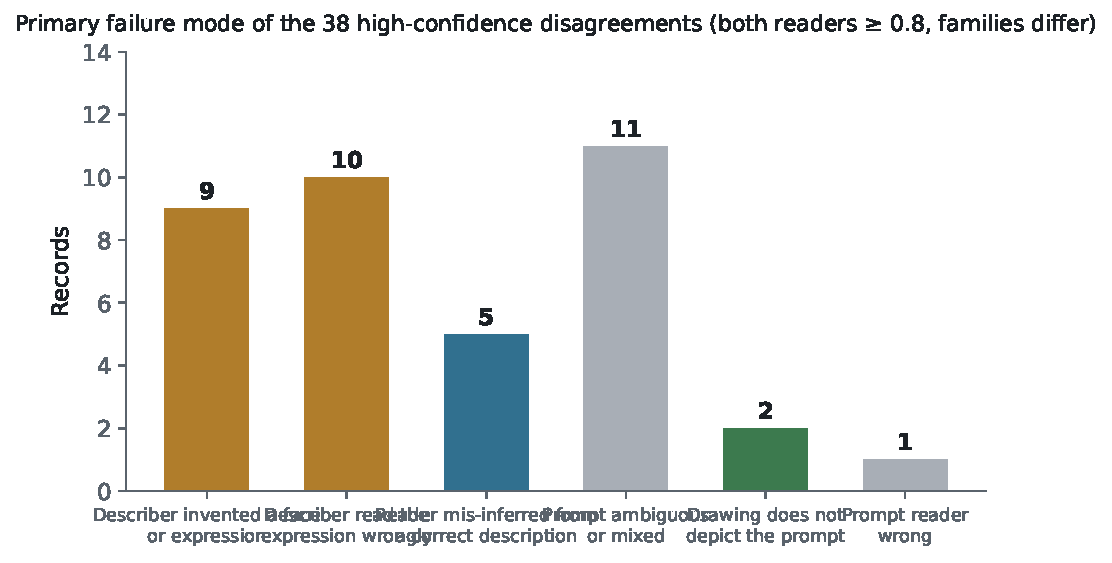
\includegraphics[width=0.95\textwidth]{fig7_error_taxonomy}
\caption{Primary failure mode of the \TaxN{} high-confidence disagreements, assigned from the drawing.}
\label{fig:taxonomy}
\end{figure}

% GENERATED by emoviz/export_tex.py — do not edit
\begin{table}[htbp]
\centering
\small
\caption{Primary failure mode of the 38 high-confidence disagreements (both readers' top-1 score $\geq 0.8$, families differ), assigned from the drawing. Describer faults (a+b) = 19; image reader (c) = 5; prompt side (d+f) = 12; generator (e) = 2.}
\label{tab:taxonomy}
\begin{tabular}{lp{0.55\textwidth}rl}
\toprule
Mode & Description & $n$ & Exemplar ids \\
\midrule
(a) & describer invented a face or expression where none is drawn & 9 & 18, 19, 242 \\
(b) & describer read the expression wrongly & 10 & 39, 192, 202 \\
(c) & reader mis-inferred from a correct description & 5 & 89, 107, 231 \\
(d) & prompt ambiguous or mixed & 11 & 65, 66, 93 \\
(e) & drawing does not depict the prompt & 2 & 137, 771 \\
(f) & prompt reader wrong & 1 & 436 \\
\bottomrule
\end{tabular}
\end{table}


\section{Description-template ablation}
\label{sec:results-ablation}

Table~\ref{tab:ablation} and Figure~\ref{fig:ablation} give the ladder under each altered template, with only the entailment stage re-run. The control re-run of the unmodified template reproduces the baseline exactly, changing the top-1 reading of \AblControlChanged{} records, so every difference in the table is a template effect and not numerical noise; the baseline row itself reproduces Section~\ref{sec:results-overall}.

Removing the expression sentence removes nearly all of the agreement. On the emotional prompts family agreement falls from \FullEmoFamObs{} to \AblDropExpressionEmoFamObs{} (null \AblDropExpressionEmoFamNull{}, $z$ = \AblDropExpressionEmoFamZ{}) and valence-sign agreement from \FullEmoSignObs{} to \AblDropExpressionEmoSignObs{} (null \AblDropExpressionEmoSignNull{}, $z$ = \AblDropExpressionEmoSignZ{}); on the face-classified records valence-sign agreement falls to \AblDropExpressionFaceSignObs{}. Fixing the expression word to ``unclear'' for every record produces the same collapse (family \AblFixedExpressionEmoFamObs{}, $z$ = \AblFixedExpressionEmoFamZ{}), and the reader's output under both variants falls to surprise or neutral for \AblDropExpressionSurprise{} and \AblDropExpressionNeutral{} of the \nAnalysed{} records respectively. Removing the action, posture or scene clause moves family agreement by one to three points (\AblDropActionEmoFamObs{}, \AblDropPostureEmoFamObs{}, \AblDropSceneEmoFamObs{}). Removing the people count raises rates and nulls together (scene valence-sign \AblDropPeopleSceneSignObs{} against \AblDropPeopleSceneSignNull{}, $z$ = \AblDropPeopleSceneSignZ{}): the ``0 people'' token pulls scene readings towards neutral, and without it the hallucinated smile is read as joy, which most prompts also are.

Under the people-aware template, which describes a drawing as ``A drawing showing \{scene\}.'' wherever the describer reports no people and leaves every other record unchanged, the face rows are identical to the baseline by construction (\AblPeopleAwareFaceSignObs{}, \AblPeopleAwareFaceFamObs{}) and the scene rows fall to their nulls: valence-sign agreement \AblPeopleAwareSceneSignObs{} against \AblPeopleAwareSceneSignNull{} ($z$ = \AblPeopleAwareSceneSignZ{}) and family agreement \AblPeopleAwareSceneFamObs{} against \AblPeopleAwareSceneFamNull{} ($z$ = \AblPeopleAwareSceneFamZ{}). Restoring the action and posture clauses to those records gives \AblPeopleAwareNoExpressionSceneSignObs{} against \AblPeopleAwareNoExpressionSceneSignNull{} ($z$ = \AblPeopleAwareNoExpressionSceneSignZ{}) and \AblPeopleAwareNoExpressionSceneFamObs{} against \AblPeopleAwareNoExpressionSceneFamNull{} ($z$ = \AblPeopleAwareNoExpressionSceneFamZ{}). Over all emotional prompts the people-aware template gives valence-sign agreement of \AblPeopleAwareEmoSignObs{} ($z$ = \AblPeopleAwareEmoSignZ{}) and family agreement of \AblPeopleAwareEmoFamObs{} ($z$ = \AblPeopleAwareEmoFamZ{}).

\begin{figure}[htbp]
\centering
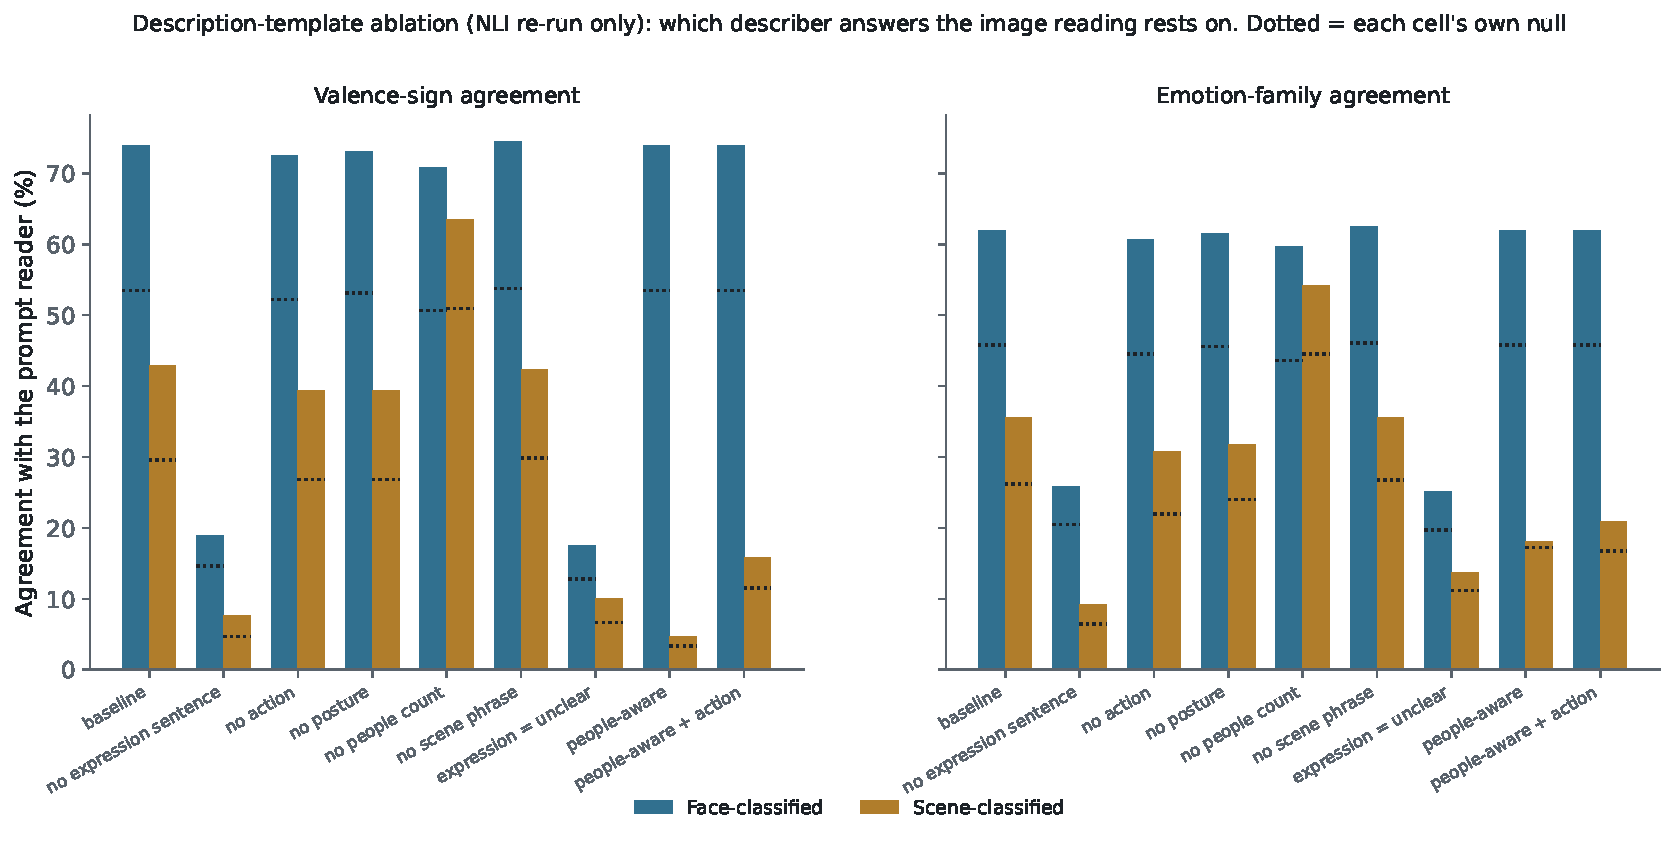
\includegraphics[width=\textwidth]{fig8_ablation}
\caption{Description-template ablation, with only the entailment stage re-run: valence-sign and family agreement by image class under each template, each bar against its own random-pairing null (dotted).}
\label{fig:ablation}
\end{figure}

% GENERATED by emoviz/export_tex.py — do not edit
\begin{table}[htbp]
\centering
\footnotesize
\caption{Description-template ablation: the NLI stage re-run on descriptions rebuilt from the cached describer answers with one clause removed or fixed; the prompt side and the null procedure unchanged. Valence-sign and family agreement per variant on the emotional prompts and their face/scene halves.}
\label{tab:ablation}
\begin{tabular}{llrrrrrrr}
\toprule
Variant & Subset & $n$ & Sign obs & null & $z$ & Family obs & null & $z$ \\
\midrule
baseline & emotional & 607 & 64.0\% & 45.6\% & +11.1 & 53.0\% & 38.8\% & +10.3 \\
 & face & 402 & 73.9\% & 53.5\% & +10.4 & 61.9\% & 45.8\% & +10.3 \\
 & scene & 205 & 42.9\% & 29.6\% & +5.8 & 35.6\% & 26.2\% & +4.4 \\
\midrule
drop\_expression & emotional & 607 & 15.3\% & 11.4\% & +5.1 & 20.3\% & 16.6\% & +3.8 \\
 & face & 402 & 18.9\% & 14.7\% & +3.8 & 25.9\% & 20.5\% & +3.8 \\
 & scene & 205 & 7.6\% & 4.7\% & +2.7 & 9.3\% & 6.4\% & +2.2 \\
\midrule
drop\_action & emotional & 607 & 61.9\% & 43.9\% & +11.0 & 50.6\% & 36.7\% & +10.3 \\
 & face & 402 & 72.5\% & 52.2\% & +10.4 & 60.7\% & 44.5\% & +10.4 \\
 & scene & 205 & 39.4\% & 26.8\% & +5.6 & 30.7\% & 21.9\% & +4.6 \\
\midrule
drop\_posture & emotional & 607 & 62.3\% & 44.5\% & +10.7 & 51.4\% & 37.9\% & +9.7 \\
 & face & 402 & 73.1\% & 53.1\% & +10.0 & 61.4\% & 45.6\% & +10.1 \\
 & scene & 205 & 39.4\% & 26.8\% & +5.6 & 31.7\% & 24.0\% & +3.6 \\
\midrule
drop\_people & emotional & 607 & 68.5\% & 50.7\% & +10.8 & 57.8\% & 43.7\% & +9.9 \\
 & face & 402 & 70.8\% & 50.7\% & +10.4 & 59.7\% & 43.6\% & +10.3 \\
 & scene & 205 & 63.5\% & 50.9\% & +5.0 & 54.1\% & 44.5\% & +3.8 \\
\midrule
drop\_scene & emotional & 607 & 64.2\% & 46.0\% & +10.7 & 53.4\% & 39.2\% & +9.8 \\
 & face & 402 & 74.4\% & 53.8\% & +10.4 & 62.4\% & 46.1\% & +10.1 \\
 & scene & 205 & 42.4\% & 29.9\% & +5.6 & 35.6\% & 26.8\% & +3.9 \\
\midrule
fixed\_expression & emotional & 607 & 15.1\% & 10.8\% & +5.9 & 21.3\% & 17.5\% & +3.9 \\
 & face & 402 & 17.5\% & 12.8\% & +4.4 & 25.1\% & 19.7\% & +4.0 \\
 & scene & 205 & 10.0\% & 6.6\% & +2.8 & 13.7\% & 11.2\% & +1.5 \\
\midrule
people\_aware & emotional & 607 & 51.7\% & 36.9\% & +10.1 & 47.1\% & 34.5\% & +8.8 \\
 & face & 402 & 73.9\% & 53.5\% & +10.4 & 61.9\% & 45.8\% & +10.3 \\
 & scene & 205 & 4.7\% & 3.4\% & +1.6 & 18.0\% & 17.3\% & +0.6 \\
\midrule
people\_aware\_no\_expression & emotional & 607 & 55.3\% & 39.5\% & +10.5 & 48.1\% & 35.0\% & +9.6 \\
 & face & 402 & 73.9\% & 53.5\% & +10.4 & 61.9\% & 45.8\% & +10.3 \\
 & scene & 205 & 15.9\% & 11.6\% & +2.7 & 21.0\% & 16.8\% & +2.2 \\
\midrule
control\_full\_template & emotional & 607 & 64.0\% & 45.6\% & +11.1 & 53.0\% & 38.8\% & +10.3 \\
 & face & 402 & 73.9\% & 53.5\% & +10.4 & 61.9\% & 45.8\% & +10.3 \\
 & scene & 205 & 42.9\% & 29.6\% & +5.8 & 35.6\% & 26.2\% & +4.4 \\
\bottomrule
\end{tabular}
\end{table}


\section{Single-coder reliability check}
\label{sec:results-human}

The 120-drawing sample has been drawn and laid out on six contact sheets (Figure~\ref{fig:codingsheet}); the coding was not complete at the time of writing, and the table in this section is generated from the scored file once it is. The table reports the describer's people count against the coder's, the face rule's precision and recall against the coder's face judgement, what lies behind the describer's ``smiling'' answers, the image reader's valence sign against the coder's, and the face/scene contrast recomputed on the coder's split rather than the describer's, which is the one estimate in the dissertation that breaks the circularity of Section~\ref{sec:method-pipeline} for the records it covers. It is a single coder, and it is stated as such.

% TODO once labels.csv is coded and `human_check.py score` has run: re-run export_tex.py, then replace this
% paragraph with the numbers (describer people-count agreement, face-rule precision/recall, smile precision,
% reader valence agreement with Wilson CIs, and the face/scene contrast on the coder's split).

% GENERATED — human check not scored when export_tex.py last ran; code outputs/human_check/labels.csv, run human_check.py score, then export_tex.py.
\noindent\emph{[Human-check table pending: code \texttt{outputs/human\_check/labels.csv}, run \texttt{human\_check.py score}, then \texttt{export\_tex.py}.]}


\section{Summary of findings}
\label{sec:results-summary}

\begin{enumerate}\setlength{\itemsep}{2pt}
\item On the \nEmotional{} prompts the text reader labels emotional, the two readers agree far above chance on every rung of the ladder: valence sign \FullEmoSignObs{} against \FullEmoSignNull{}, family \FullEmoFamObs{} against \FullEmoFamNull{}; the result survives clustering, the distinct-prompt re-run and the Holm correction (objectives 2 and 3).
\item Where the describer reports a readable face the agreement is far higher than where it reports a scene, by \DiffSignPp{} on valence sign (CI \DiffSignCi{}, $p$ = \DiffSignP{}); the scene result weakens on distinct prompts and, under a people-aware description, falls to its null (objectives 3, 4 and 7).
\item Prompts the text reader labels neutral sit at chance on the one measure that can move there, \CtrlVaObs{} against \CtrlVaNull{}, and remain there when the \CtrlFlagged{} prompts that contain an affect word are removed (objective 3).
\item Like for like, describe-then-extract agrees with the prompt reader on \McDeFam{} of families against \McClipFam{} for direct CLIP, a difference of \McDiffFamPp{} with $p$ \McClusterFamP{} on the clustered test (objective 5).
\item When the same words are drawn again, the image reader returns the same family for \ConsFam{} of drawings in a group against \ConsFamNull{} by chance ($z$ = \ConsFamZ{}): more consistent than chance and far from fixed (objective 6).
\end{enumerate}

The audits qualify all five. The describer names an expression for \DescScenePeopleZeroExpr{} of the \DescScenePeopleZero{} no-people scene records, the image reader copies an emotion-naming expression word \DescCopyStrict{} of the time, and the ablation shows that the reading rests on that word: the split and most of the agreement run through it.
